\documentclass[tikz,border=10pt]{standalone}
\usepackage[T1]{fontenc}
\usepackage[utf8]{inputenc}
\usepackage{tikz}
\usetikzlibrary{arrows.meta, positioning, calc}
% --- Same light, print-friendly palette as self-refine.tex ---
\definecolor{memFill}{HTML}{EDEEFB}\definecolor{memLine}{HTML}{4F46B8}\definecolor{memText}{HTML}{2A2461}
\definecolor{borFill}{HTML}{FBEFDB}\definecolor{borLine}{HTML}{B8791E}\definecolor{borText}{HTML}{7A4E08}
\definecolor{rewFill}{HTML}{FAECE7}\definecolor{rewLine}{HTML}{993C1D}\definecolor{rewText}{HTML}{4A1B0C}
\definecolor{movFill}{HTML}{EBF6E1}\definecolor{movLine}{HTML}{4E8A2E}\definecolor{movText}{HTML}{2E5210}
\definecolor{arrowGray}{HTML}{7A7870}\definecolor{phaseText}{HTML}{1F1F1D}
\begin{document}
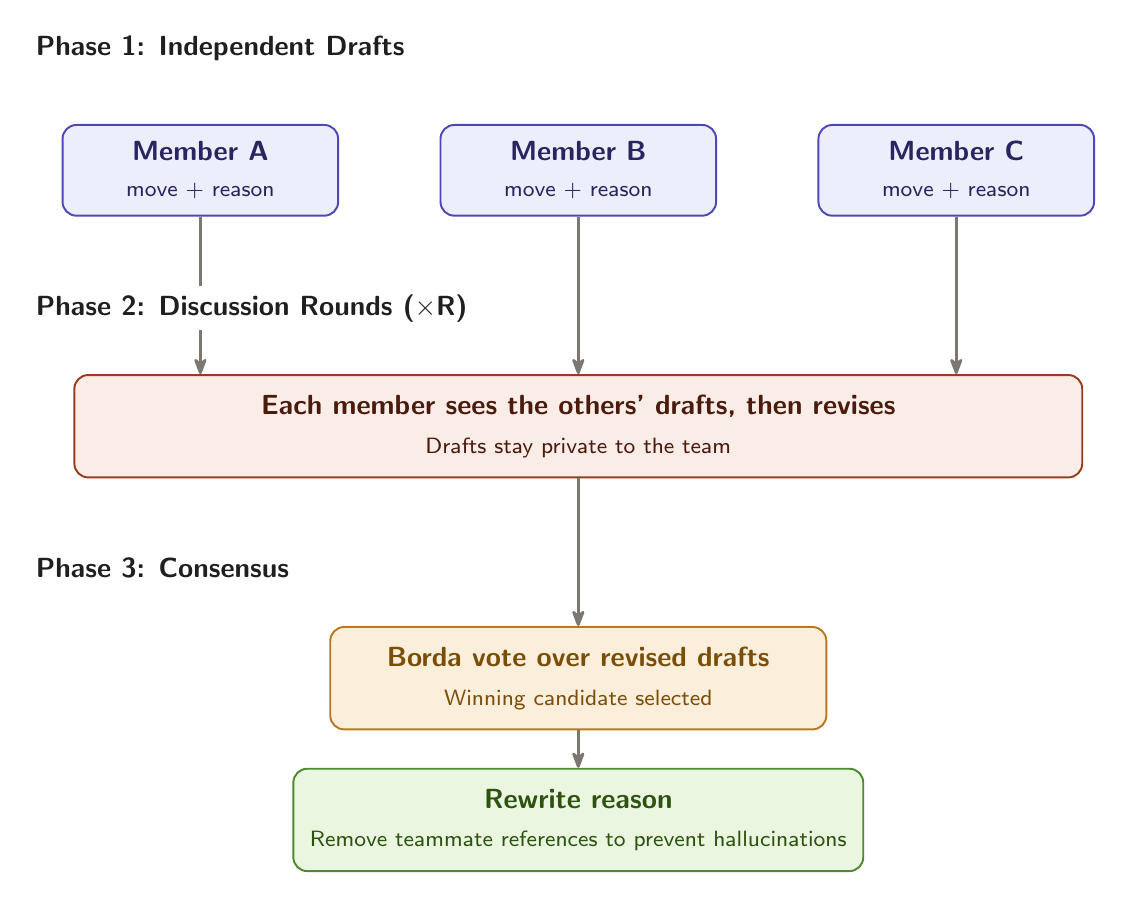
\begin{tikzpicture}[
  font=\sffamily,
  box/.style   ={rounded corners=5pt, draw, line width=0.7pt, align=center, inner sep=6pt},
  member/.style={box, fill=memFill, draw=memLine, text=memText, minimum width=3.5cm, minimum height=1.1cm},
  disc/.style  ={box, fill=rewFill, draw=rewLine, text=rewText, minimum width=12.8cm, minimum height=1.3cm},
  borda/.style ={box, fill=borFill, draw=borLine, text=borText, minimum width=6.3cm, minimum height=1.3cm},
  rew/.style   ={box, fill=movFill, draw=movLine, text=movText, minimum width=6.3cm, minimum height=1.3cm},
  phase/.style ={text=phaseText, font=\sffamily\bfseries, anchor=west, fill=white, inner sep=3pt},
  flow/.style  ={-{Stealth[round]}, draw=arrowGray, line width=1pt},
]
% ----- Phase 1 -----
\node[phase] at (-0.1,1.55) {Phase 1: Independent Drafts};
\node[member] (A) at (2.1,0)  {\textbf{Member A}\\[1pt]\footnotesize move + reason};
\node[member] (B) at (6.9,0)  {\textbf{Member B}\\[1pt]\footnotesize move + reason};
\node[member] (C) at (11.7,0) {\textbf{Member C}\\[1pt]\footnotesize move + reason};
% ----- Phase 2 -----
\node[disc] (D) at (6.9,-3.25)
  {\textbf{Each member sees the others' drafts, then revises}\\[2pt]
   \footnotesize Drafts stay private to the team};
\draw[flow] (A.south) -- (A.south |- D.north);
\draw[flow] (B.south) -- (B.south |- D.north);
\draw[flow] (C.south) -- (C.south |- D.north);
\node[phase] at (-0.1,-1.75) {Phase 2: Discussion Rounds ($\times$R)};
% ----- Phase 3 -----
\node[phase] at (-0.1,-5.05) {Phase 3: Consensus};
\node[borda] (BV) at (6.9,-6.45)
  {\textbf{Borda vote over revised drafts}\\[2pt]
   \footnotesize  Winning candidate selected};
\draw[flow] (D.south) -- (BV.north);
% ----- Reason rewrite -----
\node[rew] (RW) at (6.9,-8.25)
  {\textbf{Rewrite reason}\\[2pt]
   \footnotesize Remove teammate references to prevent hallucinations};
\draw[flow] (BV.south) -- (RW.north);
\end{tikzpicture}
\end{document}